\documentclass[tikz]{standalone}
\usepackage{tikz}

\begin{document}
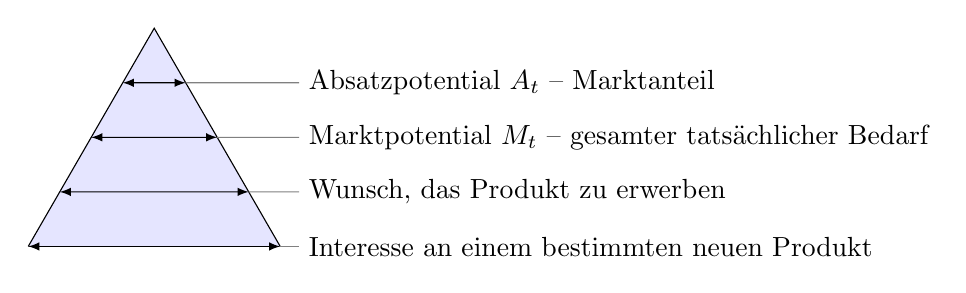
\begin{tikzpicture}[
arrow/.style={latex-latex},
label/.style={gray},
note/.style={black, right, align=left},
scale=.8
]


\draw[fill=blue!10] (0,0)--++(120:4)coordinate[pos=0](0)coordinate[pos=.25](1)coordinate[pos=.5](2)coordinate[pos=.75](3)--++(240:4)
coordinate[pos=0.25](33)coordinate[pos=.5](22)coordinate[pos=.75](11)coordinate[pos=1](00);

\path (.3,0)coordinate(GND);
\path (0)-|(GND)coordinate[midway](000);
\path (1)-|(GND)coordinate[midway](111);
\path (2)-|(GND)coordinate[midway](222);
\path (3)-|(GND)coordinate[midway](333);


\draw[arrow] (00)--(0);
\draw[arrow] (11)--(1);
\draw[arrow] (22)--(2);
\draw[arrow] (33)--(3);


\draw[label] (0)--(000) node[note]{Interesse an einem bestimmten neuen Produkt};
\draw[label] (1)--(111) node[note]{Wunsch, das Produkt zu erwerben};
\draw[label] (2)--(222) node[note]{Marktpotential $M_t$ -- gesamter tatsächlicher Bedarf};
\draw[label] (3)--(333) node[note]{Absatzpotential $A_t$ -- Marktanteil};

\end{tikzpicture}
\end{document}